\renewcommand{\thetable}{A\arabic{table}}
\renewcommand{\thefigure}{A\arabic{figure}}
\setcounter{table}{0}\setcounter{figure}{0}

\section{Tables and figures that the text refers to}\label{sec:appendix}
This appendix holds the longer tables and the further figures. Every one of them is written by a script of the repository from the unpacked session outputs in \texttt{results/raw/} (Section~\ref{sec:repro}); the tables are \texttt{report/generated/tab\_*.tex} and the figures \texttt{report/figures/}. Tables and figures of the appendix are numbered A1, A2, \ldots

\subsection{Methods and entries}
Table~\ref{tab:screen} lists every method that the screen of the newer methods considered, Table~\ref{tab:flow} the filters that led to the pool of candidates, Table~\ref{tab:entries} the twenty entries and Table~\ref{tab:pins} the pinned versions.

\begin{center}\small
\captionof{table}{Screen of newer methods (spec decision~2). \emph{Included}: \emph{baseline}, the method under test or one of the two baselines of its paper; \emph{passed}, passed the screen (CryoAtom was then dropped by the first scope cut, Section~\ref{sec:screen}); \emph{reserve}, kept in reserve and not used; \emph{no}, excluded for the reason given. The reasons are the notes written at the time of the search (to 11~October 2026).}\label{tab:screen}
\begin{longtable}{@{}p{3.0cm}p{0.9cm}p{1.5cm}p{9.0cm}@{}}
\toprule
Method & Year & Included & Reason \\
\midrule
\endfirsthead
\toprule
Method & Year & Included & Reason \\
\midrule
\endhead
\bottomrule
\endlastfoot
MICA & 2025 & baseline & {\footnotesize Method under test.} \\
ModelAngelo & 2024 & baseline & {\footnotesize One of the two methods tested in the MICA paper.} \\
EModelX(+AF) & 2024 & baseline & {\footnotesize The other method tested in the MICA paper.} \\
CryoAtom & 2025 & passed & {\footnotesize Newer than both baselines; deep learning; map + sequence to atomic model; public code and weights (MIT per README; the paper states no licence); defaults in one documented command; fits 16 GB on paper. Formerly CryFold. The CryoAtom2 preprint (proteins and nucleic acids) reports nucleic-acid results in its abstract; whether protein-only accuracy changed from v1 is not stated.} \\
EMProt & 2025 & passed & {\footnotesize Newer than both baselines; deep learning; map + sequence to atomic model; accepts per-chain predicted models, so it can take the same AF3 inputs as MICA; public code and weights; fits 16 GB on paper. Licence wording differs: README says MIT, the paper says free for academic or noncommercial users. Read the LICENSE file before release.} \\
E3-CryoFold & 2025 & passed & {\footnotesize Newer than both baselines; deep learning; map + sequence to atomic model; public code and weights (MIT per README; the paper states no licence); fits 16 GB on paper. Defaults to be taken verbatim from the README example. First excluded by mistake on an inferred link to EModelX; corrected 2026-10-11 after reading its own paper.} \\
EM3DFold & 2026 & reserve & {\footnotesize First reserve. Newer, deep learning, map + sequence to atomic model (protein-only mode available), public code and downloadable weights, fits 16 GB on paper; licence not stated. A preprint ('in submission'), so under the tie-break the three peer-reviewed methods keep their places. From the same group as EMProt; the README does not say whether it supersedes EMProt. Training-data cutoff not read: check it before use, because the benchmark relies on the 2026 entries being unseen. Recheck on 2026-10-15 for a release tag, a licence and journal status.} \\
CryoZeta & 2026 & reserve & {\footnotesize Newer, deep learning, public code and weights, but fails the 16 GB rule on paper (README: 32 GB or more) and needs MSAs from an outside tool. Second reserve, after EM3DFold: used only if EM3DFold has already replaced a method or cannot be run, and only after one pilot on the smallest entry shows it fits 16 GB.} \\
CryoACE & 2026 & no & {\footnotesize Fails the 16 GB rule (\textasciitilde{}38 GB) and is not a map-plus-sequence builder with documented defaults: it needs a rough initial model aligned to each map plus resolution and threshold settings. Its paper compares against ModelAngelo, CryoAtom, E3-CryoFold, Boltz-1 and CryoBoltz.} \\
CryoBoltz & 2025 & no & {\footnotesize Guided sampling of a Boltz model toward the map, with a pre-aligned starting model and per-map settings, not a map-plus-sequence builder with documented defaults. Also over 16 GB on the third-party figure.} \\
CryoForge & 2026 & no & {\footnotesize A post-builder correction layer that repairs another builder's model; it is not a map-plus-sequence builder. No code or weights stated.} \\
CryoNet.Discovery & 2026 & no & {\footnotesize Identifies known structures by matching map and structure embeddings (retrieval), so it does not build a model. No code or weights stated. Compared with ModelAngelo, cryoID and DomainFit.} \\
CoCoFold & 2026 & no & {\footnotesize Not a map-based builder (the input is raw particle images) and peak GPU memory is far above 16 GB. Its paper compares against DiffModeler, DeepMainmast, EModelX, MICA and ModelAngelo.} \\
Cryo2Struct & 2024 & no & {\footnotesize Not newer: published before EModelX (Nat. Commun. 15, 8808, same volume). Earlier method from the Cheng lab (Giri and Cheng); its evaluation code is checked in Phase 1 for the metric definitions.} \\
DeepMainmast & -- & no & {\footnotesize Not newer: first published online in 2023, before the ModelAngelo paper (2024).} \\
EMBuild & 2022 & no & {\footnotesize Not newer (2022).} \\
DiffModeler & 2024 & no & {\footnotesize Built for low-resolution maps; outside the <=4.0 A test range.} \\
DMcloud & 2025 & no & {\footnotesize Built for medium- to low-resolution maps; outside the <=4.0 A test range.} \\
DeepTracer (family) & -- & no & {\footnotesize Earlier family of methods; no 2025-2026 release found.} \\
CryoREAD & -- & no & {\footnotesize Models DNA and RNA only; the benchmark is protein-only.} \\
SMARTFold & 2023 & no & {\footnotesize Not newer: 2023 preprint.} \\
CryoNet.Refine & 2026 & no & {\footnotesize Refines an existing model; does not build one from a map and sequence.} \\
Cryosearch & 2026 & no & {\footnotesize Assembles components into complexes rather than building from a map and sequence; no public code found.} \\
CryoSampler & 2026 & no & {\footnotesize Models conformational ensembles; no public code found.} \\
Cryformer & -- & no & {\footnotesize Listed as its own entry in a bioRxiv review of Dec 2025 (10.64898/2025.12.28.696775; map + ESM-2 embeddings), but the name matches the encoder module of the CryFold/CryoAtom network (Cry-Net), and no separate paper or code was found.} \\
SEGEM++ & -- & no & {\footnotesize Listed in the Dec 2025 review as using AlphaFold2 output; no paper or code found under this name.} \\
Cryo2Struct2 & -- & no & {\footnotesize Described in the Dec 2025 review as map + ESM embeddings with AlphaFold3 refining its output; no paper, code or weights found under this name. How it relates to MICA is not established.} \\
CryoCodex & 2026 & no & {\footnotesize Screened by title only: map post-processing, not model building.} \\
EMAlign & 2026 & no & {\footnotesize Screened by title only: aligns cryo-EM maps, does not build models.} \\
HDOCK-Multimer & 2026 & no & {\footnotesize Screened by title only: predicts large complexes by docking and assembly; the title names no map input.} \\
Ligand-modelling paper & -- & no & {\footnotesize Screened by title only: models ligands, not protein chains.} \\
TomoSwin3D & -- & no & {\footnotesize Screened by title only: identifies and classifies macromolecules in cryo-ET tomograms, does not build models.} \\
\end{longtable}

\end{center}
\addtocounter{table}{-1}% the longtable steps the table counter once more

\begin{table}[tbp]
\centering\small
\caption{From the pool of cryo-EM entries released from 1~January to 12~October 2026 to the candidates. The map--model correlation rule and the clustering (Section~\ref{sec:datasets}) are applied to the \PoolFinal{} candidates of the last row.}
\label{tab:flow}
\fitwidth{\begin{tabular}{lrr}
\toprule
Step & Entries left & Removed \\
\midrule
Cryo-EM entries released in the window (RCSB search) & 6\,116 & -- \\
mmCIF file of at most 40 MB compressed (a larger file holds far more than 700 residues) & 6\,115 & 1 \\
PDB model released inside the window & 6\,115 & 0 \\
Single-particle reconstruction & 5\,700 & 415 \\
Resolution at most 4.0 \AA{} & 5\,219 & 481 \\
Protein only (every polymer entity is polypeptide(L)) & 3\,977 & 1\,242 \\
1 to 700 modeled residues in total & 567 & 3\,410 \\
At most 3 unique chain sequences & 548 & 19 \\
At most 5\% UNK residues & 548 & 0 \\
Exactly one EMDB map linked to the entry & 485 & 63 \\
EMDB map released inside the window (EMDB API) & 484 & 1 \\
\bottomrule
\end{tabular}
}
\end{table}

\begin{table}[tbp]
\centering\small
\caption{The twenty entries. \emph{Residues}: modelled residues of the deposit. \emph{Unique / all chains}: unique chain sequences and chains of the deposit. \emph{CC\_mask}: map--model correlation (Phenix \texttt{map\_model\_cc}, at the resolution of the entry). \emph{Max.\ identity}: highest sequence identity of any chain to a chain of a PDB entry released before 2026 (MMseqs2; 0 = no hit). \emph{AF3 pLDDT}: mean pLDDT of the AF3 predictions of the entry, weighted by residues. \emph{Map}: size of the EMDB map file.}
\label{tab:entries}
\fitwidth{\begin{tabular}{llrrcrrrr}
\toprule
PDB & EMDB & Res. (\AA) & Residues & Unique / all chains & CC\_mask & Max. identity to older PDB & AF3 pLDDT & Map (MB) \\
\midrule
\multicolumn{9}{l}{\emph{Resolution $\leq$ 3.0 \AA}} \\
9T5K & 55586 & 2.60 & 381 & 1 / 1 & 0.82 & 0.61 & 85 & 250 \\
22FX & 68251 & 1.24 & 173 & 1 / 1 & 0.74 & 1.00 & 97 & 75 \\
9JKK & 61564 & 3.00 & 530 & 1 / 1 & 0.84 & 1.00 & 85 & 66 \\
9TKA & 56022 & 2.70 & 247 & 1 / 1 & 0.76 & 0.00 & 88 & 182 \\
9WFL & 65930 & 2.75 & 682 & 2 / 2 & 0.84 & 1.00 & 91 & 66 \\
9VI4 & 65077 & 1.80 & 516 & 1 / 1 & 0.87 & 0.98 & 98 & 1024 \\
9ZLH & 74403 & 2.14 & 206 & 1 / 1 & 0.85 & 1.00 & 92 & 66 \\
9VUH & 65363 & 2.70 & 634 & 3 / 3 & 0.74 & 1.00 & 77 & 128 \\
9OC0 & 70305 & 2.97 & 512 & 2 / 4 & 0.83 & 1.00 & 84 & 333 \\
13BD & 76936 & 2.65 & 461 & 1 / 2 & 0.88 & 0.95 & 84 & 281 \\
\midrule
\multicolumn{9}{l}{\emph{Resolution $>$ 3.0 to 4.0 \AA}} \\
9WQ6 & 66160 & 3.40 & 261 & 1 / 1 & 0.76 & 1.00 & 84 & 128 \\
9V4D & 64777 & 3.07 & 276 & 2 / 2 & 0.82 & 0.50 & 71 & 54 \\
9OTA & 70828 & 3.20 & 534 & 1 / 2 & 0.85 & 1.00 & 86 & 69 \\
9KQM & 62507 & 3.50 & 403 & 1 / 1 & 0.79 & 1.00 & 76 & 66 \\
9WME & 66088 & 3.20 & 446 & 2 / 2 & 0.70 & 1.00 & 90 & 23 \\
9VBD & 64920 & 3.26 & 521 & 1 / 1 & 0.77 & 0.00 & 93 & 128 \\
9RWS & 54346 & 3.28 & 512 & 1 / 1 & 0.85 & 0.44 & 88 & 128 \\
9WTX & 66226 & 3.37 & 500 & 1 / 1 & 0.72 & 0.76 & 88 & 128 \\
9Z24 & 73762 & 3.10 & 338 & 1 / 1 & 0.87 & 1.00 & 80 & 221 \\
26DK & 80558 & 3.50 & 191 & 1 / 1 & 0.74 & 0.00 & 97 & 16 \\
\bottomrule
\end{tabular}
}
\end{table}

\begin{table}[tbp]
\centering\small
\caption{Pinned versions of the methods and the tools, as recorded in the run information of the sessions.}
\label{tab:pins}
\fitwidth{\begin{tabular}{ll}
\toprule
Component & Commit or file (pinned) \\
\midrule
MICA & \texttt{726d1bb14be04887a43b7f5aefcff0d843761d01} \\
ModelAngelo & \texttt{994945bdfa6e5368e0d62349a47792f4864eebc3} \\
EModelX(+AF) & \texttt{53713cf820d10d78b1ca6669ef197850cf907843} \\
EMProt & \texttt{9489d52e7fdc81c85ba82e386abcfa05bac2b9d1} \\
E3-CryoFold & \texttt{241cef48da83b96519e62ab02cccd9db96d8e68b} \\
Phenix & \texttt{Phenix-2.2.1-6174-Linux-x86\_64.sh} \\
US-align & \texttt{746ad8a2a4dea9f317075cc482df0ecb5440bdea} \\
\bottomrule
\end{tabular}
}
\end{table}

\subsection{Sessions, docking and failures}
Table~\ref{tab:sessions} lists the sessions, Table~\ref{tab:docking} the docking of every entry in the three passes, Table~\ref{tab:modes} MICA's outcome by entry and Table~\ref{tab:failures} every failed run.

\begin{table}[tbp]
\centering\small
\caption{The \NSessions{} Kaggle sessions that produced results (CPU sessions have no GPU). Status of the entries of a session: \emph{ok}, finished with its output; \emph{docked}, programs 1 and 2 of MICA finished and the docked state was saved for a GPU session; \emph{failed}, ended without the output of its step; \emph{deferred}, program 3 of MICA was switched off after two failures in a row and the entry waits; \emph{interrupted}, cut by the end of the session; \emph{killed\_corun}, a baseline killed by the system while the other GPU was busy (it ran again alone, Section~\ref{sec:procedure}); \emph{not run}, no work was started. The baseline sessions count runs (method $\times$ entry), the MICA sessions count entries, and the scoring sessions the models that they scored. The result of \texttt{mica\_cpu\_c} for 9VUH (pass~1) is not used: every MICA result comes from the pass-3 set-up.}
\label{tab:sessions}
\fitwidth{\begin{tabular}{llrcl}
\toprule
Notebook & Started (UTC) & Minutes & GPU & Entries by status, or models scored \\
\midrule
\texttt{gpu\_batch1} & 2026-10-23 05:35 & 521 & yes & ok 64, failed 3, killed\_corun 6, not run 7 \\
\texttt{mica\_cpu\_a} & 2026-10-24 06:34 & 417 & no & failed 3, deferred 4 \\
\texttt{gpu\_batch2} & 2026-10-24 06:44 & 410 & yes & ok 1, failed 4, interrupted 1, not run 7 \\
\texttt{mica\_cpu\_c} & 2026-10-24 06:40 & 441 & no & ok 1, failed 4, deferred 1 \\
\texttt{mica\_cpu\_b} & 2026-10-24 06:37 & 611 & no & failed 5, deferred 2 \\
\texttt{mica\_dock2\_a} & 2026-10-25 16:17 & 262 & no & docked 4, failed 1 \\
\texttt{mica\_dock2\_d} & 2026-10-25 16:23 & 284 & no & docked 2, failed 3 \\
\texttt{mica\_dock2\_b} & 2026-10-25 16:19 & 377 & no & failed 5 \\
\texttt{mica\_dock2\_c} & 2026-10-25 16:21 & 379 & no & docked 1, failed 4 \\
\texttt{gpu\_batch3} & 2026-10-25 16:30 & 432 & yes & ok 6, failed 2 \\
\texttt{mica\_dock3\_c} & 2026-10-26 10:46 & 229 & no & docked 5 \\
\texttt{mica\_dock3\_a} & 2026-10-26 10:42 & 272 & no & docked 5 \\
\texttt{mica\_dock3\_d} & 2026-10-26 10:48 & 275 & no & docked 5 \\
\texttt{mica\_dock3\_b} & 2026-10-26 10:44 & 459 & no & docked 5 \\
\texttt{scoring\_base} & 2026-10-27 02:08 & 26 & no & 127 models scored \\
\texttt{mica\_gpu\_nodock} & 2026-10-27 02:05 & 105 & yes & ok 8, failed 3, deferred 9 \\
\texttt{mica\_gpu} & 2026-10-27 02:04 & 143 & yes & ok 8, failed 3, deferred 9 \\
\texttt{scoring\_mica} & 2026-10-27 10:15 & 14 & no & 24 models scored \\
\texttt{scoring\_nodock} & 2026-10-27 10:18 & 14 & no & 24 models scored \\
\texttt{mica\_gpu2\_b} & 2026-10-27 16:38 & 190 & yes & ok 6, failed 1 \\
\texttt{mica\_gpu2\_a} & 2026-10-27 16:34 & 195 & yes & ok 3, interrupted 2 (cut by the time budget) \\
\texttt{scoring\_mica2} & 2026-10-28 05:45 & 17 & no & 27 models scored \\
\texttt{mica\_gpu3} & 2026-10-28 05:02 & 186 & yes & failed 2 \\
\bottomrule
\end{tabular}
}
\end{table}

\begin{table}[tbp]
\centering\small
\caption{Docking of the AF3 domains in the three passes (Section~\ref{sec:dockprocedure}): domains docked of the domains found by Merizo, and the median local correlation (CC) of the docked domains. The correlations of pass~1 and pass~3 are not comparable (pass~3 is measured at 6~\AA{} after a coarse refinement). \emph{Mode}: docking mode of the entry in pass~3. The last row sums the domains of the 20 entries; its CC is the median over all docked domains of the pass.}
\label{tab:docking}
\fitwidth{\begin{tabular}{lrccccccl}
\toprule
Entry & Domains & Pass 1 docked & CC & Pass 2 docked & CC & Pass 3 docked & CC & Mode \\
\midrule
9T5K & 2 & 1 / 2 & 0.47 & 1 / 2 & 0.47 & 1 / 2 & 0.11 & partial \\
22FX & 2 & 0 / 2 & -- & 0 / 2 & -- & 1 / 2 & 0.09 & partial \\
9JKK & 2 & 0 / 2 & -- & 0 / 2 & -- & 2 / 2 & 0.11 & full \\
9TKA & 1 & 1 / 1 & 0.44 & 1 / 1 & 0.44 & 1 / 1 & 0.08 & full \\
9WFL & 5 & 1 / 5 & 0.47 & 1 / 5 & 0.47 & 5 / 5 & 0.06 & full \\
9VI4 & 3 & 0 / 3 & -- & 0 / 3 & -- & 0 / 3 & -- & none \\
9ZLH & 2 & 0 / 2 & -- & 0 / 2 & -- & 2 / 2 & 0.10 & full \\
9VUH & 4 & 4 / 4 & 0.42 & 4 / 4 & 0.42 & 4 / 4 & 0.17 & full \\
9OC0 & 7 & 0 / 7 & -- & 0 / 7 & -- & 3 / 7 & 0.05 & partial \\
13BD & 3 & 2 / 3 & 0.21 & 0 / 3 & -- & 1 / 3 & 0.06 & partial \\
9WQ6 & 1 & 0 / 1 & -- & 0 / 1 & -- & 1 / 1 & 0.03 & full \\
9V4D & 1 & 0 / 1 & -- & 0 / 1 & -- & 1 / 1 & 0.09 & full \\
9OTA & 2 & 0 / 2 & -- & 0 / 2 & -- & 2 / 2 & 0.10 & full \\
9KQM & 2 & 1 / 2 & 0.08 & 1 / 2 & 0.08 & 2 / 2 & 0.07 & full \\
9WME & 7 & 2 / 7 & 0.46 & 2 / 7 & 0.46 & 7 / 7 & 0.08 & full \\
9VBD & 4 & 0 / 4 & -- & 0 / 4 & -- & 4 / 4 & 0.11 & full \\
9RWS & 3 & 0 / 3 & -- & 0 / 3 & -- & 3 / 3 & 0.09 & full \\
9WTX & 3 & 0 / 3 & -- & 0 / 3 & -- & 3 / 3 & 0.10 & full \\
9Z24 & 3 & 0 / 3 & -- & 0 / 3 & -- & 1 / 3 & 0.14 & partial \\
26DK & 2 & 2 / 2 & 0.53 & 2 / 2 & 0.53 & 2 / 2 & 0.27 & full \\
\midrule
All & 59 & 14 / 59 & 0.44 & 12 / 59 & 0.45 & 46 / 59 & 0.09 &  \\
\bottomrule
\end{tabular}
}
\end{table}

\begin{table}[tbp]
\centering\small
\caption{MICA by entry: domains, domains docked in pass~3, docking mode, outcome of program~3 (\emph{failed $\to$ ok}: the first attempt failed with a GPU out-of-memory error and the rerun with the memory patch built the model) and TM-score of the model (F: no model).}
\label{tab:modes}
\fitwidth{\begin{tabular}{lrrlll}
\toprule
Entry & Domains & Docked & Mode & Program 3 & TM-score \\
\midrule
9T5K & 2 & 1 & partial & ok & 0.80 \\
22FX & 2 & 1 & partial & failed $\to$ ok & 0.98 \\
9JKK & 2 & 2 & full & ok & 0.99 \\
9TKA & 1 & 1 & full & ok & 0.99 \\
9WFL & 5 & 5 & full & ok & 0.95 \\
9VI4 & 3 & 0 & none & failed & F \\
9ZLH & 2 & 2 & full & ok & 0.99 \\
9VUH & 4 & 4 & full & ok & 0.96 \\
9OC0 & 7 & 3 & partial & failed & F \\
13BD & 3 & 1 & partial & ok & 0.88 \\
9WQ6 & 1 & 1 & full & failed $\to$ ok & 0.90 \\
9V4D & 1 & 1 & full & failed $\to$ ok & 0.94 \\
9OTA & 2 & 2 & full & ok & 0.91 \\
9KQM & 2 & 2 & full & ok & 0.93 \\
9WME & 7 & 7 & full & ok & 0.94 \\
9VBD & 4 & 4 & full & ok & 0.98 \\
9RWS & 3 & 3 & full & ok & 0.94 \\
9WTX & 3 & 3 & full & ok & 0.93 \\
9Z24 & 3 & 1 & partial & ok & 0.90 \\
26DK & 2 & 2 & full & failed & F \\
\bottomrule
\end{tabular}
}
\end{table}

\begin{table}[tbp]
\centering\small
\caption{Every run that ended without a scored model, with the reason recorded by the notebook. Exit code $-9$ is a kill by the system.}
\label{tab:failures}
\fitwidth{\begin{tabular}{@{}lllp{9.4cm}@{}}
\toprule
Entry & Method & Outcome & Reason (from the status table) \\
\midrule
13BD & E3-CryoFold & failed & prealign: exit code 1; the model file 13BD\_e3\_prealign.pdb was not written \\
13BD & CryoAtom & failed & build: out of GPU memory (exit code 1; the error message of the program); the model file 13BD\_cryoatom1.cif was not written \\
13BD & CryoZeta & failed & run: out of GPU memory (exit code 2; the error message of the program); the model file 13BD\_sample\_0.cif was not written \\
26DK & MICA & failed & 3\_build: exit code -9; the output of 3\_build was not written \\
26DK & EModelX(+AF) & failed & temp\_flex: killed by the system (exit code -9, probably out of memory); the model file 26dk\_EModelX(+AF)\_all\_atom\_model.pdb was not written \\
26DK & E3-CryoFold & failed & prealign: killed by the system (exit code -9, probably out of memory); the model file 26DK\_e3\_prealign.pdb was not written \\
26DK & CryoZeta & failed & run: killed by the system (exit code -9, probably out of memory; also when it ran alone); the model file 26DK\_sample\_0.cif was not written \\
9OC0 & MICA & failed & 3\_build: timeout after 7200 s; the output of 3\_build was not written \\
9OC0 & E3-CryoFold & failed & prealign: exit code 1; the model file 9OC0\_e3\_prealign.pdb was not written \\
9OC0 & CryoAtom & failed & build: out of GPU memory (exit code 1; the error message of the program); the model file 9OC0\_cryoatom1.cif was not written \\
9OC0 & CryoZeta & failed & run: killed by the system (exit code -9, probably out of memory; also when it ran alone); the model file 9OC0\_sample\_0.cif was not written \\
9OTA & E3-CryoFold & failed & prealign: exit code 1; the model file 9OTA\_e3\_prealign.pdb was not written \\
9VBD & CryoAtom & failed & build: out of GPU memory (exit code 1; the error message of the program); the model file 9VBD\_cryoatom1.cif was not written \\
9VBD & CryoZeta & failed & run: timeout: the run limit of 21600 s; the model file 9VBD\_sample\_0.cif was not written \\
9VI4 & MICA & failed & 3\_build: exit code -9; the output of 3\_build was not written \\
9VI4 & ModelAngelo & failed & build: timeout: the run limit of 10800 s; the model file 9VI4\_modelangelo.cif was not written \\
9VI4 & EModelX(+AF) & failed & temp\_flex: killed by the system (exit code -9, probably out of memory); the model file 9vi4\_EModelX(+AF)\_all\_atom\_model.pdb was not written \\
9VI4 & EMProt & failed & build: killed by the system (exit code -9, probably out of memory); the model file output.cif was not written \\
9VI4 & E3-CryoFold & failed & prealign: killed by the system (exit code -9, probably out of memory); the model file 9VI4\_e3\_prealign.pdb was not written \\
9VI4 & CryoZeta & not run & killed\_corun: killed by the system (exit code -9, probably out of memory) while the other GPU's program ran; run again alone \\
9VUH & CryoZeta & failed & run: timeout: the run limit of 21600 s; the model file 9VUH\_sample\_0.cif was not written \\
9WFL & CryoZeta & not run & interrupted: stopped by the end of the session after 17039 s; run again in the next session \\
9WME & CryoZeta & not run & interrupted: stopped by the end of the session after 17022 s; run again in the next session \\
9Z24 & CryoAtom & failed & build: out of GPU memory (exit code 1; the error message of the program); the model file 9Z24\_cryoatom1.cif was not written \\
9Z24 & CryoZeta & failed & run: timeout: the run limit of 21600 s; the model file 9Z24\_sample\_0.cif was not written \\
\bottomrule
\end{tabular}
}
\end{table}

\subsection{Further results}
Tables~\ref{tab:zero} and~\ref{tab:dockeffect} belong to Sections~\ref{sec:results} (failures as zero) and~\ref{sec:dockresults} (docked input); the other tables give the TM-score of every method on every entry (Table~\ref{tab:perentry}), all measures (Tables~\ref{tab:allmetrics}, \ref{tab:strata} and~\ref{tab:fns}), the other output files of the methods (Table~\ref{tab:variants}), the correlations (Table~\ref{tab:corr}), the run times (Table~\ref{tab:runtime}) and the comparison with MICA without docked input (Table~\ref{tab:pairednodock}).

\begin{table}[tbp]
\centering\small
\caption{Failed runs scored as zero: mean TM-score over all 20 entries and the paired comparison with MICA. The two policies give the same means and tests because every run was either scored or failed; the intervals can differ in the last digit because the bootstrap draws differ.}
\label{tab:zero}
\fitwidth{\begin{tabular}{lrcrrr}
\toprule
Method & $n$ & Mean TM-score [95\% CI] & Mean diff. to MICA & Wilcoxon $p$ & Holm $p$ \\
\midrule
\multicolumn{6}{l}{\emph{Failed and unusable runs scored 0 (runs not made are left out)}} \\
MICA & 20 & 0.80 [0.64, 0.93] & -- & -- & -- \\
ModelAngelo & 20 & 0.76 [0.62, 0.88] & $-$0.04 & 0.738 & 1.000 \\
EModelX(+AF) & 20 & 0.84 [0.70, 0.94] & 0.05 & 0.551 & 1.000 \\
EMProt & 20 & 0.91 [0.80, 0.98] & 0.12 & $<$0.001 & $<$0.001 \\
E3-CryoFold & 20 & 0.65 [0.46, 0.81] & $-$0.15 & 0.002 & 0.005 \\
\midrule
\multicolumn{6}{l}{\emph{Every missing result scored 0}} \\
MICA & 20 & 0.80 [0.64, 0.93] & -- & -- & -- \\
ModelAngelo & 20 & 0.76 [0.62, 0.88] & $-$0.04 & 0.738 & 1.000 \\
EModelX(+AF) & 20 & 0.84 [0.70, 0.94] & 0.05 & 0.551 & 1.000 \\
EMProt & 20 & 0.91 [0.80, 0.98] & 0.12 & $<$0.001 & $<$0.001 \\
E3-CryoFold & 20 & 0.65 [0.47, 0.81] & $-$0.15 & 0.002 & 0.005 \\
\bottomrule
\end{tabular}
}
\end{table}

\begin{table}[tbp]
\centering\small
\caption{MICA with and without docked AF3 input on the entries that ran in both set-ups (difference = docked minus no docked input).}
\label{tab:dockeffect}
\fitwidth{\begin{tabular}{lrlccr}
\toprule
Entry & Res. (\AA) & Docking & TM docked & TM no docked input & Difference \\
\midrule
9JKK & 3.00 & full & 0.995 & 0.991 & +0.004 \\
9WFL & 2.75 & full & 0.954 & 0.954 & 0.000 \\
9ZLH & 2.14 & full & 0.994 & 0.994 & 0.000 \\
9VUH & 2.70 & full & 0.956 & 0.909 & +0.047 \\
9OTA & 3.20 & full & 0.913 & 0.913 & +0.001 \\
9KQM & 3.50 & full & 0.929 & 0.856 & +0.073 \\
9WME & 3.20 & full & 0.941 & 0.929 & +0.012 \\
9RWS & 3.28 & full & 0.943 & 0.942 & +0.001 \\
\midrule
\multicolumn{6}{l}{Mean difference 0.017 [0.002, 0.037]; median 0.002; Wilcoxon $p$ = 0.039; higher / lower / equal: 6 / 2 / 0} \\
\bottomrule
\end{tabular}
}
\end{table}

\begin{table}[tbp]
\centering\small
\caption{TM-score of every method on every entry (normalised by the deposited model; F: failed run).}
\label{tab:perentry}
\fitwidth{\begin{tabular}{lrccccccc}
\toprule
Entry & Res. (\AA) & MICA & ModelAngelo & EModelX(+AF) & EMProt & E3-CryoFold & CryoAtom & CryoZeta \\
\midrule
\multicolumn{9}{l}{\emph{Resolution $\leq$ 3.0 \AA}} \\
9T5K & 2.60 & 0.80 & 1.00 & 0.99 & 1.00 & 0.68 & 1.00 & 0.94 \\
22FX & 1.24 & 0.98 & 1.00 & 0.97 & 1.00 & 0.97 & 1.00 & 0.98 \\
9JKK & 3.00 & 0.99 & 0.99 & 0.99 & 1.00 & 0.98 & 1.00 & 1.00 \\
9TKA & 2.70 & 0.99 & 1.00 & 0.99 & 1.00 & 0.98 & 1.00 & 0.99 \\
9WFL & 2.75 & 0.95 & 0.99 & 0.95 & 0.99 & 0.98 & 1.00 & N \\
9VI4 & 1.80 & F & F & F & F & F & 1.00 & N \\
9ZLH & 2.14 & 0.99 & 1.00 & 0.99 & 0.99 & 0.96 & 1.00 & 0.99 \\
9VUH & 2.70 & 0.96 & 0.75 & 0.91 & 0.97 & 0.63 & 0.86 & F \\
9OC0 & 2.97 & F & 0.78 & 0.86 & 0.67 & F & F & F \\
13BD & 2.65 & 0.88 & 0.98 & 0.92 & 0.99 & F & F & F \\
\midrule
\multicolumn{9}{l}{\emph{Resolution $>$ 3.0 to 4.0 \AA}} \\
9WQ6 & 3.40 & 0.90 & 0.45 & 0.89 & 0.94 & 0.80 & 0.53 & 0.98 \\
9V4D & 3.07 & 0.94 & 0.58 & 0.94 & 0.95 & 0.91 & 0.96 & 0.98 \\
9OTA & 3.20 & 0.91 & 0.91 & 0.93 & 0.98 & F & 0.97 & 0.98 \\
9KQM & 3.50 & 0.93 & 0.79 & 0.86 & 0.96 & 0.90 & 0.63 & 0.99 \\
9WME & 3.20 & 0.94 & 0.56 & 0.84 & 0.95 & 0.60 & 0.78 & N \\
9VBD & 3.26 & 0.98 & 0.24 & 0.99 & 0.99 & 0.97 & F & F \\
9RWS & 3.28 & 0.94 & 0.97 & 0.96 & 0.98 & 0.96 & 0.99 & 0.99 \\
9WTX & 3.37 & 0.93 & 0.27 & 0.93 & 0.98 & 0.73 & 0.61 & 0.99 \\
9Z24 & 3.10 & 0.90 & 0.90 & 0.91 & 0.91 & 0.89 & F & F \\
26DK & 3.50 & F & 0.95 & F & 0.98 & F & 0.98 & F \\
\bottomrule
\end{tabular}
}
\end{table}

\begin{table}[tbp]
\centering\small
\caption{Median (interquartile range) of every measure (Table~\ref{tab:metrics}) over the scored models of each method. The sets of entries differ between methods.}
\label{tab:allmetrics}
\fitwidth{\begin{tabular}{lccccc}
\toprule
Metric & MICA & ModelAngelo & EModelX(+AF) & EMProt & E3-CryoFold \\
\midrule
TM-score & 0.94 (0.91--0.98) & 0.91 (0.67--0.99) & 0.94 (0.91--0.98) & 0.98 (0.96--0.99) & 0.91 (0.77--0.97) \\
C$\alpha$ match (\%) & 94.9 (86.0--96.3) & 91.1 (48.0--98.5) & 94.1 (90.1--97.6) & 57.4 (21.8--90.2) & 80.9 (69.2--96.9) \\
Sequence match (\%) & 98.5 (96.5--99.7) & 98.8 (98.1--99.8) & 97.4 (87.3--99.4) & 98.5 (96.5--99.7) & 96.0 (75.5--98.3) \\
Coverage & 1.02 (1.00--1.05) & 1.01 (0.89--2.06) & 1.01 (0.98--1.04) & 1.45 (1.08--4.59) & 1.03 (1.00--1.16) \\
C$\alpha$ quality (\%) & 96.0 (94.2--97.9) & 96.7 (80.5--99.5) & 94.7 (91.4--98.1) & 98.2 (94.6--99.7) & 92.0 (80.0--98.9) \\
Aligned sequence identity (\%) & 99.3 (97.8--99.7) & 99.5 (98.3--99.9) & 98.7 (96.3--99.6) & 99.5 (97.5--100.0) & 98.3 (86.2--99.8) \\
RMSD (\AA) & 1.10 (0.68--1.28) & 0.63 (0.39--0.94) & 1.02 (0.78--1.66) & 0.92 (0.41--1.30) & 1.44 (1.05--2.40) \\
Aligned length & 409 (265--495) & 306 (179--468) & 428 (276--501) & 393 (260--513) & 309 (252--470) \\
\bottomrule
\end{tabular}
}
\end{table}

\begin{table}[tbp]
\centering\small
\caption{TM-score by resolution stratum: entries, scored models, median (interquartile range) and mean with 95\,\% bootstrap CI.}
\label{tab:strata}
\fitwidth{\begin{tabular}{lrrcc}
\toprule
Method & Entries & Models & Median (IQR) & Mean [95\% CI] \\
\midrule
\multicolumn{5}{l}{\emph{Resolution $\leq$ 3.0 \AA}} \\
MICA & 10 & 8 & 0.97 (0.93--0.99) & 0.94 [0.89, 0.98] \\
ModelAngelo & 10 & 9 & 0.99 (0.98--1.00) & 0.94 [0.87, 1.00] \\
EModelX(+AF) & 10 & 9 & 0.97 (0.92--0.99) & 0.95 [0.92, 0.98] \\
EMProt & 10 & 9 & 0.99 (0.99--1.00) & 0.96 [0.88, 1.00] \\
E3-CryoFold & 10 & 7 & 0.97 (0.82--0.98) & 0.88 [0.77, 0.98] \\
\midrule
\multicolumn{5}{l}{\emph{Resolution $>$ 3.0 to 4.0 \AA}} \\
MICA & 10 & 9 & 0.93 (0.91--0.94) & 0.93 [0.92, 0.95] \\
ModelAngelo & 10 & 10 & 0.68 (0.47--0.91) & 0.66 [0.49, 0.82] \\
EModelX(+AF) & 10 & 9 & 0.93 (0.89--0.94) & 0.92 [0.89, 0.94] \\
EMProt & 10 & 10 & 0.97 (0.95--0.98) & 0.96 [0.95, 0.98] \\
E3-CryoFold & 10 & 8 & 0.90 (0.78--0.92) & 0.85 [0.76, 0.92] \\
\bottomrule
\end{tabular}
}
\end{table}

\begin{table}[tbp]
\centering\small
\caption{Fragment-agnostic TM-score (US-align \texttt{-mm 5}): median (interquartile range) over the scored models, and the paired comparison with MICA on the entries where both built a model (method minus MICA; Wilcoxon $p$ and its Holm correction over the four methods).}
\label{tab:fns}
\fitwidth{\begin{tabular}{lrcccc}
\toprule
Method & $n$ & TM-score, fragment-agnostic, median (IQR) & Mean difference to MICA [95\% CI] & Wilcoxon $p$ & Holm $p$ \\
\midrule
MICA & 17 & 0.96 (0.94--0.98) & -- & -- & -- \\
ModelAngelo & 19 & 0.96 (0.82--0.99) & $-$0.07 [$-$0.14, $-$0.00] & 0.243 & 0.487 \\
EModelX(+AF) & 18 & 0.95 (0.93--0.98) & 0.00 [$-$0.01, 0.03] & 0.464 & 0.487 \\
EMProt & 19 & 0.99 (0.98--0.99) & 0.03 [0.01, 0.05] & 0.002 & 0.007 \\
E3-CryoFold & 15 & 0.93 (0.84--0.97) & $-$0.05 [$-$0.08, $-$0.02] & 0.002 & 0.007 \\
\bottomrule
\end{tabular}
}
\end{table}

\begin{table}[tbp]
\centering\small
\caption{Further output files of each method, scored with the same protocol next to the file of the main comparison (marked \emph{scored}); $n$ is the number of entries with the file. Only the file marked \emph{scored} is used in the comparisons.}
\label{tab:variants}
\fitwidth{\begin{tabular}{@{}p{5.2cm}r*{6}{>{\raggedleft\arraybackslash}p{1.45cm}}@{}}
\toprule
Output & $n$ & TM-score, median & TM-score, mean & Fragment-agnostic TM, median & C$\alpha$ match, median & Coverage, median & C$\alpha$ quality, median \\
\midrule
MICA, all-atom model (scored) & 17 & 0.94 & 0.94 & 0.96 & 94.9 & 1.02 & 96.0 \\
MICA, C$\alpha$ model after chain building & 17 & 0.94 & 0.94 & 0.96 & 94.9 & 1.02 & 96.2 \\
MICA, initial C$\alpha$ model of the network & 17 & 0.82 & 0.82 & 0.86 & 99.5 & 0.86 & 84.4 \\
ModelAngelo, sequence-assigned model (scored) & 19 & 0.91 & 0.79 & 0.96 & 91.1 & 1.01 & 96.7 \\
ModelAngelo, model without sequence assignment & 19 & 0.50 & 0.50 & 0.99 & 48.5 & 1.47 & 98.2 \\
EModelX(+AF), all-atom model (scored) & 18 & 0.94 & 0.94 & 0.95 & 94.1 & 1.01 & 94.7 \\
EModelX(+AF), C$\alpha$ model & 18 & 0.94 & 0.94 & 0.95 & 94.1 & 1.01 & 94.7 \\
EMProt, build with the AF3 models (scored) & 19 & 0.98 & 0.96 & 0.99 & 57.4 & 1.45 & 98.2 \\
EMProt, de novo model & 19 & 0.96 & 0.82 & 0.97 & 97.2 & 1.00 & 97.1 \\
E3-CryoFold, \texttt{pre\_align} model (scored) & 15 & 0.91 & 0.86 & 0.93 & 80.9 & 1.03 & 92.0 \\
CryoAtom v1.0.0, pruned model (scored) & 16 & 0.98 & 0.89 & 0.99 & 76.7 & 1.16 & 99.2 \\
CryoAtom v1.0.0, model before pruning & 16 & 0.78 & 0.75 & 0.99 & 36.7 & 2.04 & 99.8 \\
CryoZeta, top-ranked sample 0 (scored) & 11 & 0.99 & 0.98 & 0.99 & 84.3 & 1.17 & 98.8 \\
CryoZeta, sample 1 (ranked second) & 11 & 0.99 & 0.98 & 0.99 & 84.3 & 1.17 & 99.3 \\
CryoZeta, sample 2 (ranked third) & 11 & 0.99 & 0.98 & 0.99 & 84.3 & 1.17 & 99.0 \\
CryoZeta, sample 3 (ranked fourth) & 11 & 0.99 & 0.98 & 0.99 & 85.5 & 1.17 & 98.9 \\
CryoZeta, sample 4 (ranked fifth) & 11 & 0.99 & 0.98 & 0.99 & 84.3 & 1.17 & 98.8 \\
\bottomrule
\end{tabular}
}
\end{table}

\begin{table}[tbp]
\centering\small
\caption{Spearman rank correlation (two-sided $p$ in brackets, not corrected for multiple tests) of the TM-score with the resolution of the map, the number of modelled residues and the highest identity to older PDB entries; $n$ is the number of scored models.}
\label{tab:corr}
\fitwidth{\begin{tabular}{lrccc}
\toprule
Method & $n$ & Resolution & Modelled residues & Identity to older PDB \\
\midrule
MICA & 17 & $-$0.25 (0.325) & 0.03 (0.896) & 0.02 (0.940) \\
ModelAngelo & 19 & $-$0.66 (0.002) & $-$0.29 (0.237) & 0.05 (0.835) \\
EModelX(+AF) & 18 & $-$0.48 (0.044) & $-$0.18 (0.463) & $-$0.42 (0.080) \\
EMProt & 19 & $-$0.53 (0.018) & $-$0.13 (0.609) & $-$0.28 (0.247) \\
E3-CryoFold & 15 & $-$0.28 (0.305) & $-$0.00 (0.990) & $-$0.11 (0.685) \\
CryoAtom & 16 & $-$0.79 ($<$0.001) & $-$0.14 (0.617) & $-$0.10 (0.715) \\
CryoZeta & 11 & 0.11 (0.750) & 0.19 (0.574) & $-$0.25 (0.462) \\
\bottomrule
\end{tabular}
}
\end{table}

\begin{table}[tbp]
\centering\small
\caption{Wall-clock time per run (failed runs included). For MICA it is the time of programs 1 to 3 including docking; the baselines ran with another program on the second GPU of the session, so the times are indicative.}
\label{tab:runtime}
\fitwidth{\begin{tabular}{lrrrrl}
\toprule
Method & Runs & Median (min) & Range (min) & Total (h) & Device \\
\midrule
MICA & 20 & 81.6 & 32.8--557.5 & 40.0 & cuda \\
ModelAngelo & 20 & 20.3 & 7.9--180.0 & 12.2 & 0, 1 \\
EModelX(+AF) & 20 & 6.9 & 2.4--96.8 & 4.8 & 0, 1 \\
EMProt & 20 & 14.2 & 4.6--58.5 & 7.0 & 0, 1 \\
E3-CryoFold & 20 & 2.9 & 1.0--20.3 & 1.7 & 0, 1 \\
\bottomrule
\end{tabular}
}
\end{table}

\begin{table}[tbp]
\centering\small
\caption{Paired comparison of the TM-score with MICA run without docked input, on the entries where that run and the method both have a model (method minus MICA; as Table~\ref{tab:paired}).}
\label{tab:pairednodock}
\fitwidth{\begin{tabular}{lrccrrrc}
\toprule
Method & Pairs & Mean difference [95\% CI] & Median diff. & Wilcoxon $p$ & Holm $p$ & $t$-test Holm $p$ & higher / lower / equal \\
\midrule
\multicolumn{8}{l}{\emph{All entries}} \\
ModelAngelo & 8 & $-$0.07 [$-$0.17, 0.01] & 0.00 & 0.461 & 1.000 & 0.884 & 4 / 4 / 0 \\
EModelX(+AF) & 8 & $-$0.01 [$-$0.03, 0.01] & 0.00 & 0.617 & 1.000 & 0.884 & 4 / 4 / 0 \\
EMProt & 8 & 0.04 [0.02, 0.07] & 0.04 & 0.016 & 0.094 & 0.061 & 7 / 1 / 0 \\
E3-CryoFold & 7 & $-$0.08 [$-$0.20, 0.02] & $-$0.01 & 0.578 & 1.000 & 0.884 & 3 / 4 / 0 \\
CryoAtom & 8 & $-$0.03 [$-$0.10, 0.03] & 0.00 & 0.844 & 1.000 & 0.884 & 5 / 3 / 0 \\
CryoZeta & 5 & 0.05 [0.01, 0.09] & 0.05 & 0.125 & 0.625 & 0.528 & 4 / 1 / 0 \\
\midrule
\multicolumn{8}{l}{\emph{Resolution $\leq$ 3.0 \AA}} \\
ModelAngelo & 4 & $-$0.03 [$-$0.12, 0.03] & 0.00 & 0.875 & 1.000 & 1.000 & 3 / 1 / 0 \\
EModelX(+AF) & 4 & 0.00 [$-$0.00, 0.00] & 0.00 & 0.750 & 1.000 & 1.000 & 1 / 3 / 0 \\
EMProt & 4 & 0.03 [0.00, 0.05] & 0.02 & 0.250 & 1.000 & 1.000 & 3 / 1 / 0 \\
E3-CryoFold & 4 & $-$0.07 [$-$0.21, 0.01] & $-$0.02 & 0.375 & 1.000 & 1.000 & 1 / 3 / 0 \\
CryoAtom & 4 & $-$0.00 [$-$0.04, 0.03] & 0.00 & 0.875 & 1.000 & 1.000 & 3 / 1 / 0 \\
CryoZeta & 2 & 0.00 [$-$0.00, 0.01] & 0.00 & 1.000 & 1.000 & 1.000 & 1 / 1 / 0 \\
\midrule
\multicolumn{8}{l}{\emph{Resolution $>$ 3.0 to 4.0 \AA}} \\
ModelAngelo & 4 & $-$0.10 [$-$0.28, 0.01] & $-$0.04 & 0.375 & 1.000 & 1.000 & 1 / 3 / 0 \\
EModelX(+AF) & 4 & $-$0.01 [$-$0.06, 0.02] & 0.01 & 0.875 & 1.000 & 1.000 & 3 / 1 / 0 \\
EMProt & 4 & 0.06 [0.03, 0.09] & 0.05 & 0.125 & 0.750 & 0.248 & 4 / 0 / 0 \\
E3-CryoFold & 3 & $-$0.09 [$-$0.33, 0.04] & 0.02 & 1.000 & 1.000 & 1.000 & 2 / 1 / 0 \\
CryoAtom & 4 & $-$0.07 [$-$0.18, 0.05] & $-$0.05 & 0.625 & 1.000 & 1.000 & 2 / 2 / 0 \\
CryoZeta & 3 & 0.08 [0.05, 0.13] & 0.07 & 0.250 & 1.000 & 0.365 & 3 / 0 / 0 \\
\bottomrule
\end{tabular}
}
\end{table}

\subsection{Further figures}
The figures show the distributions of the measures (Figures~\ref{fig:dist} and~\ref{fig:allmetrics}), the pairs of TM-scores (Figure~\ref{fig:pairs}), the outcomes and the run times (Figures~\ref{fig:outcomes} and~\ref{fig:runtime}), and the checks with the fragment-agnostic score and the resolution (Figures~\ref{fig:frag}, \ref{fig:res} and~\ref{fig:pairedfns}).

\begin{figure}[tbp]
\centering
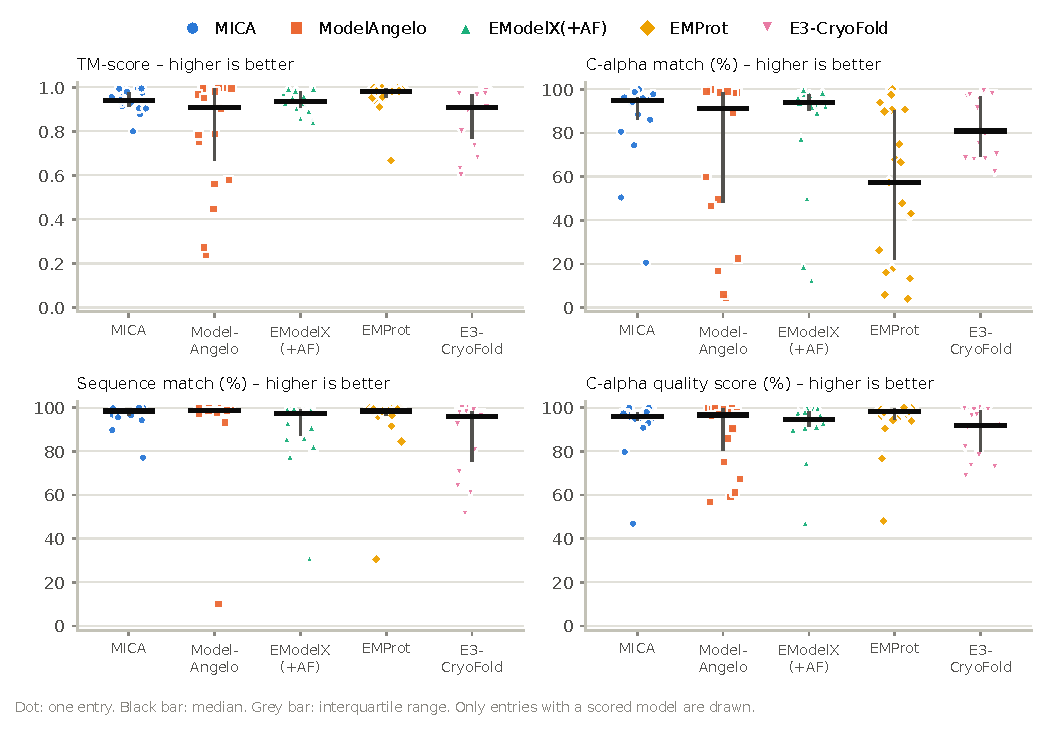
\includegraphics[width=\textwidth]{figures/fig4_distributions.pdf}
\caption{Four measures over the scored models of each method (one dot per entry; black bar: median; grey bar: interquartile range).}
\label{fig:dist}
\end{figure}

\begin{figure}[tbp]
\centering
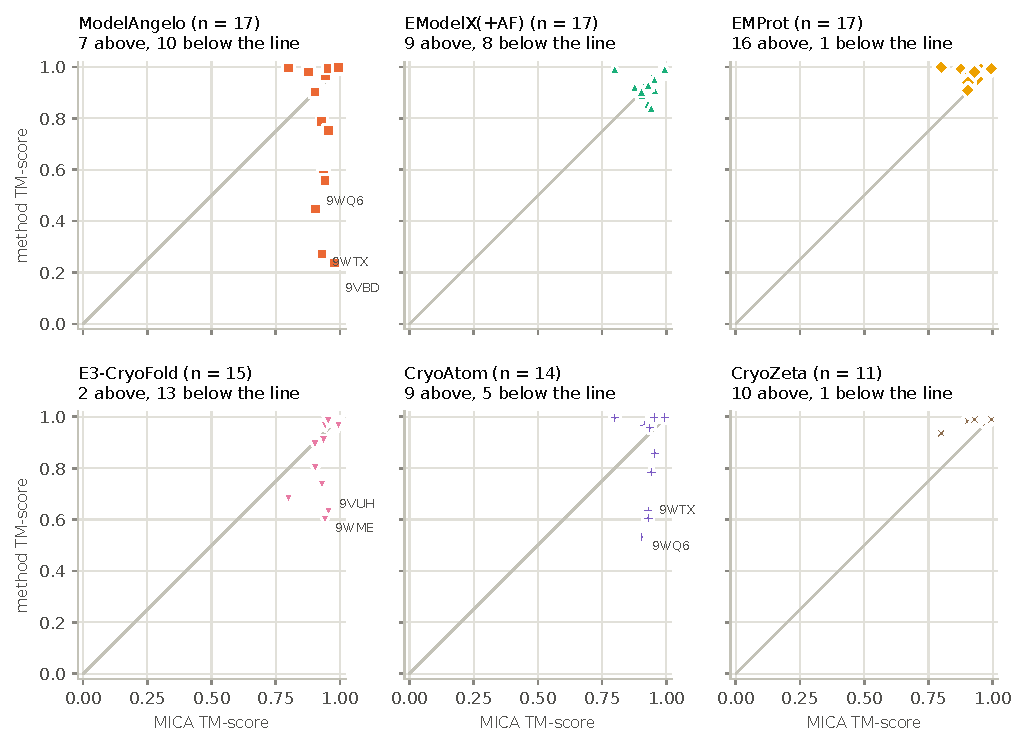
\includegraphics[width=\textwidth]{figures/fig3_tm_score_pairs.pdf}
\caption{TM-score of each method against that of MICA on the same entry (the line is equality; entries that differ by 0.3 or more are labelled, at most three per panel).}
\label{fig:pairs}
\end{figure}

\begin{figure}[tbp]
\centering
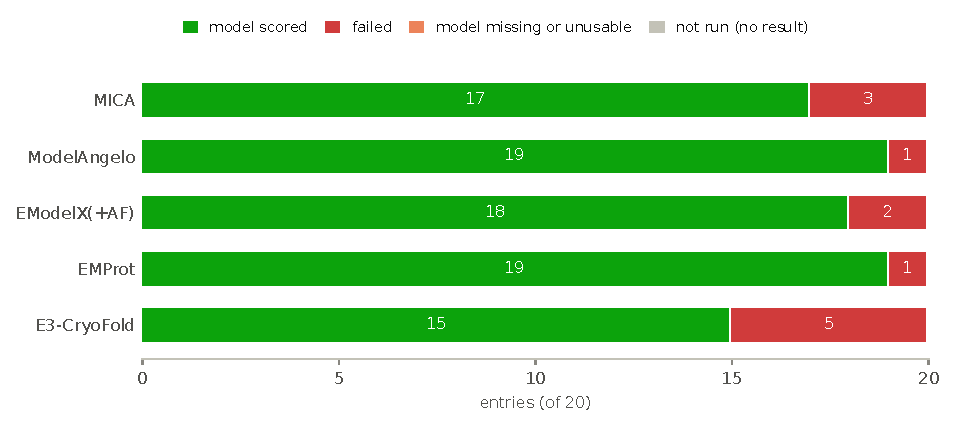
\includegraphics[width=0.85\textwidth]{figures/fig5_outcomes.pdf}
\caption{Outcome of the 20 runs of each method.}
\label{fig:outcomes}
\end{figure}

\begin{figure}[tbp]
\centering
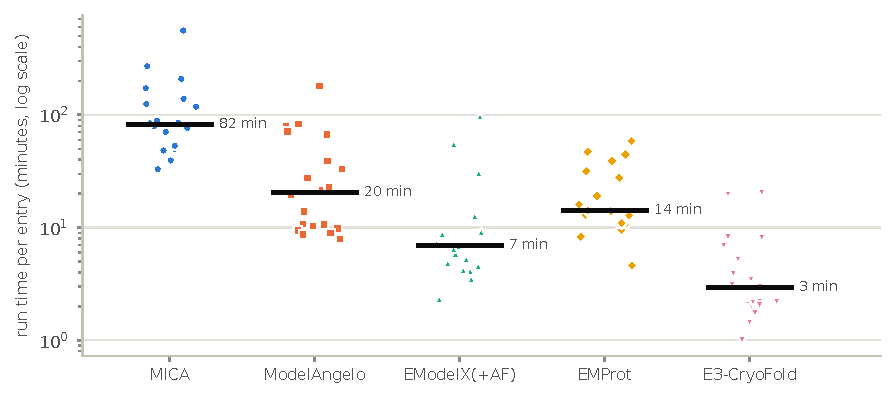
\includegraphics[width=0.8\textwidth]{figures/fig6_runtime.pdf}
\caption{Run time of every run (failed runs included; logarithmic axis); the bar is the median.}
\label{fig:runtime}
\end{figure}

\begin{figure}[tbp]
\centering
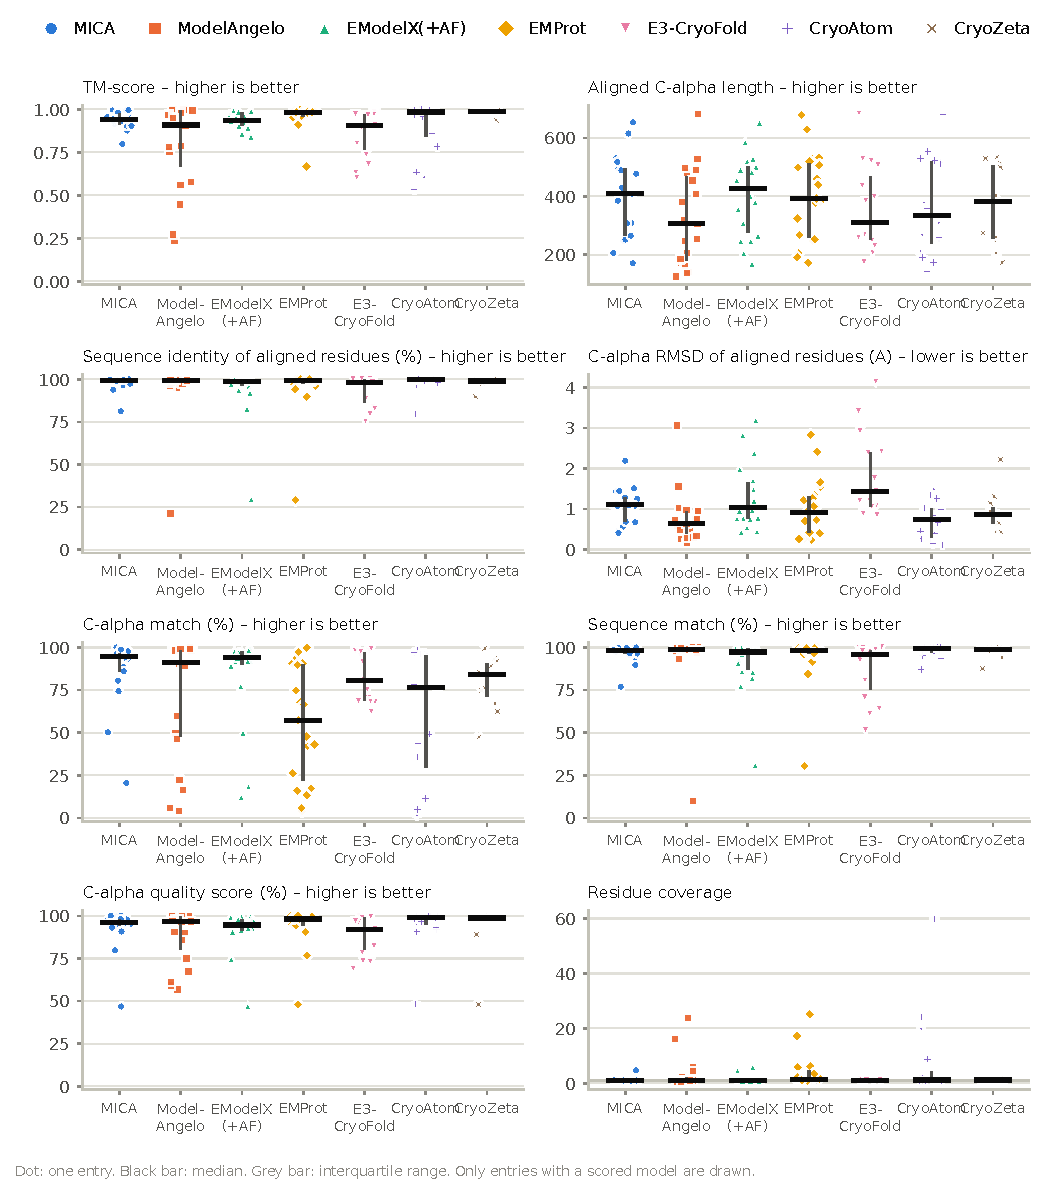
\includegraphics[width=\textwidth]{figures/figA1_all_metrics.pdf}
\caption{All measures over the scored models of each method (as Figure~\ref{fig:dist}).}
\label{fig:allmetrics}
\end{figure}

\begin{figure}[tbp]
\centering
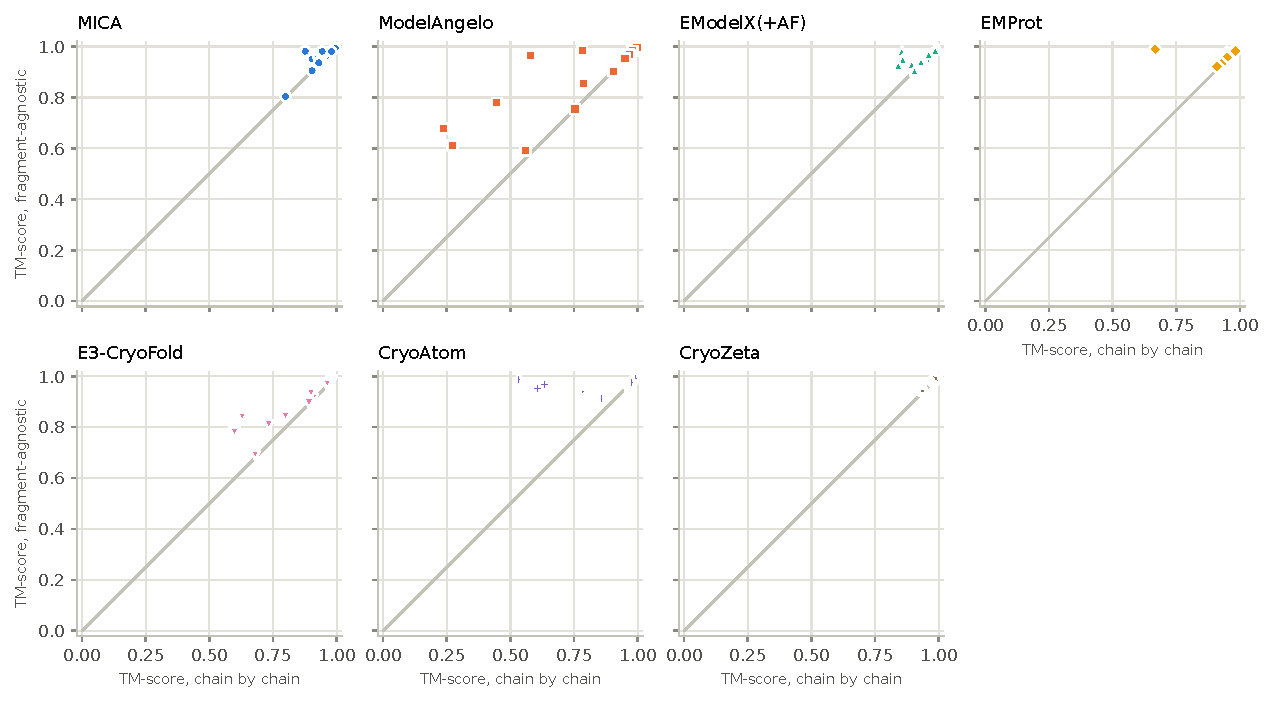
\includegraphics[width=\textwidth]{figures/figA2_fragmentation.pdf}
\caption{TM-score chain by chain (the primary measure) against the fragment-agnostic TM-score. A point above the line is a model whose primary score is lowered by fragmentation or by extra chains.}
\label{fig:frag}
\end{figure}

\begin{figure}[tbp]
\centering
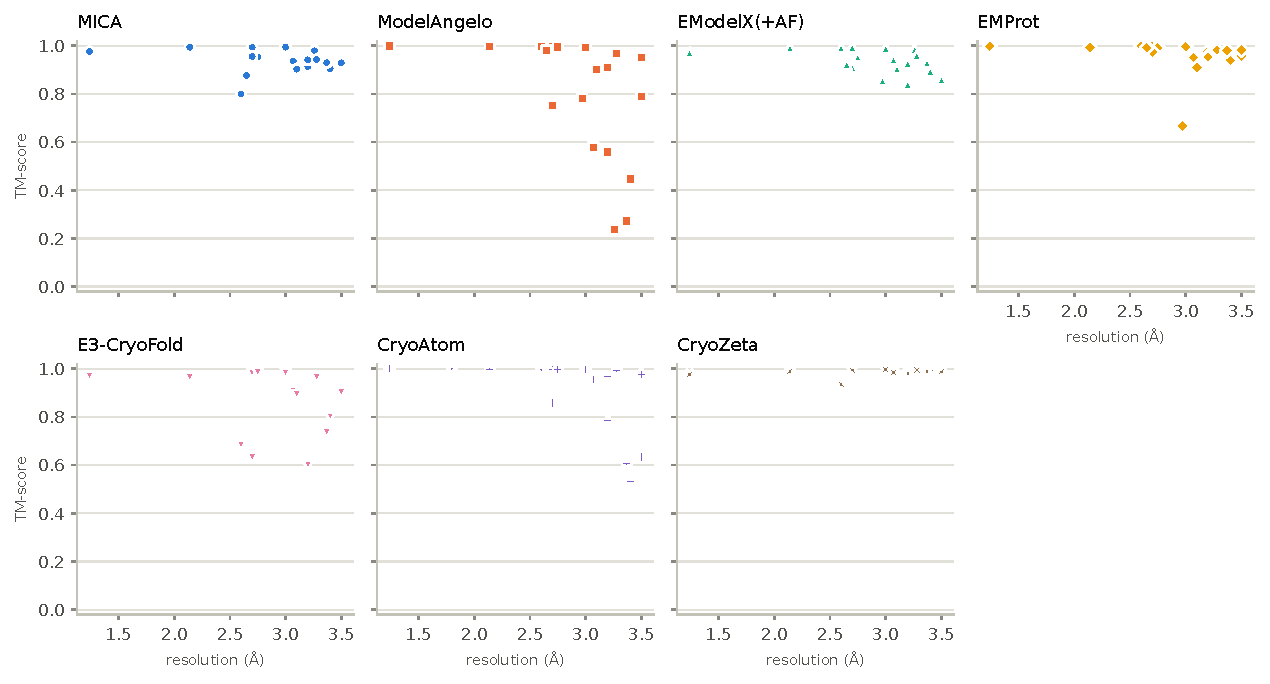
\includegraphics[width=\textwidth]{figures/figA3_resolution.pdf}
\caption{TM-score of each method against the resolution of the map.}
\label{fig:res}
\end{figure}

\begin{figure}[tbp]
\centering
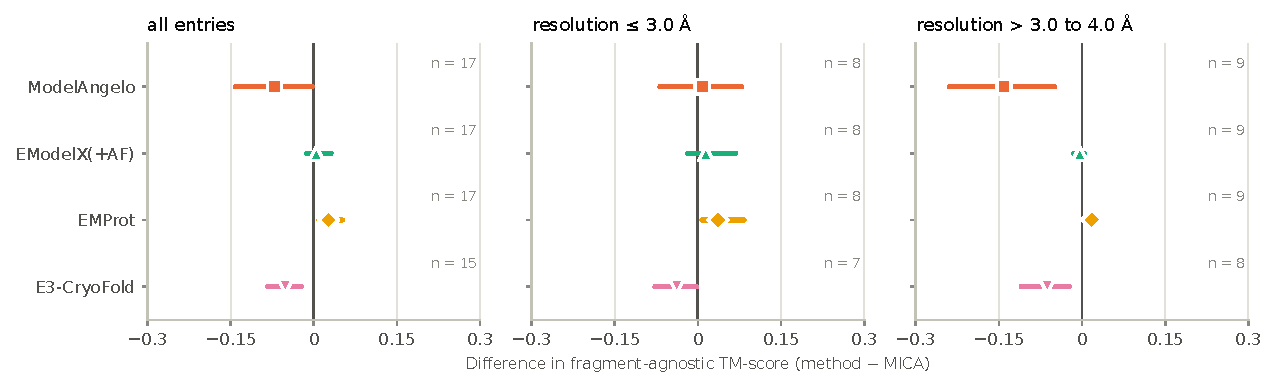
\includegraphics[width=\textwidth]{figures/figA4_paired_differences_fragment_agnostic.pdf}
\caption{Difference between each method and MICA in the fragment-agnostic TM-score (as Figure~\ref{fig:paired}).}
\label{fig:pairedfns}
\end{figure}
